
\begin{definition}{Functional equivalence:}
    \label{def:semantic_equivalence}
    Let P and P' two programs, P and P' are functionally equivalent if given the same input both programs produce the same output.
    
    Notice that by definition, P is semantically equivalent to P itself. Besides, this definition is sound with the definition of equivalence module input of Lee \etal \cite{}.
\end{definition}

Let us have the space of all possible programs that can be constructed under a given language. A diversifier can be defined as a searching problem, \ie given a program in this space, search all other programs that are functionally equivalent to it. The found programs are called variants. Notice that, the concept of functional equivalence is subjective by nature. For example, two programs can be functionally equivalent module input but in terms of performance they might not be considered equivalent. In the majority of the cases \cite{}, a program variant is only considered under equivalence modulo input \cite{}.

% TODO, extend this with why a theorem prover is needed, why not based on unit tests ?
The problem of searching for program variants is challenging for obvious reasons. First, this space is infinite and checking all possible programs for those equivalent variants is algorithmically impossible. Second, the equivalence checking is expensive because a theorem prover is needed to prove that two programs are fully equivalent \cite{}.

Program optimization during compiling can be seen as a subproblem, \ie given a program, to find the best equivalent program in all the program's space. Compilers usually solve this problem by changing the original program following known transformation rules that are known move this search from a program to a smaller one in terms on number of instructions. 


\begin{definition}{Code transformation:}
    \label{def:code_transformation}
    TODO
\end{definition}

This process is then followed with the result foundlings until no it cannot find another smaller program. 


All this said, the very first premise to find program variants is that the found variants should be semantically equivalent, \ie every time a program variant is executed with the same input as the original program, both should return the same result. In terms of wording, we can say that the programs are not created, but they are found in the large space of all possible programs. 


\begin{definition}{Program variant:}
    \label{def:variant}
    Let P and P' two programs, P' is a variant of P if, according to the \autoref{def:semantic_equivalence}, they are functionally equivalent.
\end{definition}
    

With the previous definitions we enunciate what a diversifier should be in \autoref{alg:diversifier}:


\begin{algorithm}[H]

    \SetKwData{optimizations}{optimizations}
    \SetKwData{variants}{variants}
    \SetKwData{B}{P'}
    \SetKwData{subset}{subset}
    \SetKwFunction{so}{sop}
    \SetKwFunction{variantfrom}{variant from}
    \SetKwFunction{to}{to}
    \SetKwInOut{Input}{input}\SetKwInOut{Output}{output}
    \Input{program $P$}
    \Output{Collection of program variants \variants }
    $\variants \leftarrow \emptyset$ \;
    \While{True}{
        \B $\leftarrow$ \variantfrom $P$\;   
        \If{\B and $P$ are semantically equivalent}{
            \variants $\leftarrow$ \variants $+$ \B\;
        }
    }
    
    \caption{Program diversifier}
\label{alg:diversifier}

\end{algorithm}

A program variant can be created by transforming the original program. This transformation must be consequent with the defined functional equivalence rule. 
XXX and YYY proposed to solve this issue by using the optimization options already available in the compilers. For example, by applying a set of the compiler optimizations during the compilation of the original program, the variants are created by changing out code that it not the best in terms of performance. The result of the transformations is a program that behaves as the original program but faster. 

% Extend this into a paragraph
The main limitation with this approach is that the number of programs that can be generated from all compiler option combinations are finite. The key challenge then, is to find a way to remove the limits on the number of variants that can be generated. This limit is the definition of compiler optimization.  Imagine the space of all possible program variants, the compiler just take care about those programs that are better than the original in terms of performance.


\section{A superdiversifier}

Given a program, code superoptimization produces new program variant, functionally equivalent to the original but better according to a concrete criterion. For example, a superoptimizer would try to generate a program variant with fewer instructions or that produces a smaller compiled binary \cite{1987_Massalin_Sueroptimizer}. Superoptimizers first detect all \emph{optimizations}. Optimizations are the pieces of code that could be replaced by a functionally equivalent code fragment, ensuring an improvement of the criterion. A \emph{superoptimized} program will result from applying all these replacements or optimizations at once. Thus, this process could be defined in the algorithm proposed in \autoref{gen:algorthm}


We leverage the search strategy of superoptimizers to generate several variants of a given program. Our main idea is to generate a new program variant by applying a subset of the optimizations found by a superoptimizer. Our proposal is summarized in \autoref{alg:generation}. We consider the superoptimization search strategy to be a function that takes as input a program, and returns the set of all possible optimizations for a concrete criterion. Once the superoptimizer has detected all possible optimizations, we build the \emph{power set} of all these replacements. Then, we apply, in turn, all the optimization subsets in this power set. The application of the optimizations in the subset will generate a new program variant. Notice that, applying the empty subset produces the original program and applying the set of all optimizations is equivalent to \emph{superoptimizing} the original program. Thus, these two variants are also produced by our strategy.


%In this section, we discuss key concepts and we enumerate the definitions used along this chapter. 

%\subsubsection{WebAssembly}


% Probably to be moved to introduction
%WebAssemblyis a binary instruction format for a stack-based virtual machine. It addresses the issues of being safe, fast, portable and compact low-level code on the web. The language was first published in 2015 \cite{}, formalized then by Haas \etal \cite{} and since 2020 it was officially accepted as the four web language \cite{}. Further the web development, WebAssemblyhas been used in standalone environments, given it is platform-agnostic \cite{}.

\section{Superdiversifier}

\section{Souper}

\section{Methodology}

\section{CROW}

\subsection{Functional equivalence}

In this section, we define and discuss the concept of functional equivalence, code transformation and program variant.



\subsection{Static}
\subsection{Dynamic}
\subsection{Preservation}

We translate each \wasm\ multivariant binary with Lucet, to determine the impact of this translation to machine code on the function variants and the diversity of paths in the multivariant call graph. 

% Description of the table and general stats
The 'x86 code' section of \autoref{table:CFG1} summarizes the key data to answer RQ2. Column \#Variants shows the number of preserved variants in the x86 code of each endpoint, column \#Paths shows the number of possible paths in the x86 multivariant binary. The last two columns show  the ratio of paths (PP) and variants (PV) preserved in x86. 
Note that the path preservation ratio metric is a projection of the variant preservation and the call graph in the multivariant binary.

 
% Previous works and why some functions have several preserved transformations
In all cases, more than 77\% of the individual function variants present in the multivariant Wasm  binary are preserved in the x86 multivariant. This high preservation rate for function variants allows to preserve a large ratio of possible paths in the multivariant call graph.
In 4 out of 7 cases, more than 83\% of the possible execution paths in the multivariant WebAssemblybinary are preserved.
The translation to machine code preserves 21\% and 17\% of the possible paths for \texttt{qr\_str} and \texttt{qr\_image}. Yet, the x86 version of the multiversion call graph for these endpoints still includes millions of possible paths, with 17 and 15 randomization points. The translation to machine drastically reduces the potential for randomized execution paths only for \texttt{bin2base64}, for which it preserves only 25\% of the possible paths, for a total of 41 paths.

% Population's compression
We have identified why some variants are not preserved the translation from Wasm  to x86. Lucet performs optimization passes before generating machine code. 
In some cases, this can annihilate the effect of CROW's diversification transformation. 
For example, in \autoref{mul:prevalence_example}, CROW synthesizes a variant in the right column by splitting it in two  multiplications relying on the integer overflow mechanism. 
A  constant merging optimization pass could remove the constant multiplications by performing it at compilation time. 
The other transformation cases that we have observed have the same property, the transformations are simple enough to be quickly verified at compilation time.

\lstset{
    language=WAT,
    style=WATStyle,
    stepnumber=0,
    label=EQExample}
\begin{code}
\noindent\begin{minipage}[b]{0.9\linewidth}
    
    \begin{minipage}[t]{0.45\linewidth}
        \begin{lstlisting}
; previous stack code;
i32.const -10
i32.mul
        \end{lstlisting}
    \end{minipage}%
    \hfill\noindent\begin{minipage}[t]{0.45\linewidth}
       
        \begin{lstlisting}
; previous stack code ;
i32.const -1931544174
i32.mul
i32.const 109653155
i32.mul
        \end{lstlisting}
    \end{minipage}
    
    %\noindent\rule{\linewidth}{0.4pt}
    \captionof{lstlisting}{Two examples of block variants that are functionally equivalent and implement with different \wasm\ instructions. The variant on the left, generated by \tool, is not preserved through the translation to machine code.}\label{mul:prevalence_example}
\end{minipage}
\end{code}





We identified where the optimizations are done in Lucet's compiler, \footnote{\url{https://github.com/bytecodealliance/wasmtime/blob/main/cranelift/codegen/src/preopt.peepmatic} and \url{https://github.com/bytecodealliance/wasmtime/blob/main/cranelift/codegen/src/postopt.rs}}. It performs optimization-like transformations that are simpler than the ones introduced by CROW. 
With this result we also encourage to avoid the usage of the insertion of \texttt{nop} instructions either in Wasm  or machine code. \texttt{nop} operations could be easily detected and removed by a latter optimization stage.



Moreover, the last three endpoints have a path preservation ratio that is less than 0.25, even with more than 87\%  of individual function  variants that are preserved. This is explained by the fact that the number of possible paths is related to both the number of variants and to the complexity of the call graph.

\todo{Add image}


The example in \autoref{diag:preservation}  illustrates this phenomenon.
Suppose an original binary composed of three functions with the call graph illustrated at the top of the figure. Here, we count 2 possible paths (one with no iteration, and one with a single iteration).
\tool generates 2 variants for $f2$ and 4 variants for $f3$, the multivariant wasm call graph is illustrated at the center of the figure. The number of possible execution paths increases to 40.
In the translation process, Lucet transforms the two \wasm\ function variants for $f2$ into the same x86 function.
In this case, the number of possible execution paths in the x86 multivariant call graph is reduced by a factor of 2, from 40 to 20.
However, the number of variants is decreased only in 1. 
The complexity of the call graph has a major impact on the number of possible execution paths. 


	The translation from \wasm\ to machine code through Lucet preserves a high ratio of function variants. This leads to the preservation of high numbers of possible execution paths in the multivariant binaries. 
	Our multivariant execution scheme is appropriate for the state-of-the-art runtime of edge computing nodes.


\section{Conclusions}

\todo{One figure per RQ result, and one big explanation.}

\todo{Remove all except dynamic comparison.}

\todo{For RQ2, focus more on preservationa and refer to contribution on the first twoe ones.}



\begin{comment}
    This section describes CROW, a tool tailored to create semantically equivalent variants out of a single program, either C/C++ code or LLVM bitcode. We assume that the \wasm\ programs are generated through the LLVM compilation pipeline to implement CROW. This assumption is supported by the work of Lehman et al. \cite{}; the fact that LLVM-based compilers are the most popular compilers to build \wasm\ programs \cite{usenixWASM2020} and the availability of source code (typically C/C++; and LLVM for \wasm) that provides a structure to perform code analysis and produce code replacements that is richer than the binary code. CROW is part of the contributions of this thesis.
    In \autoref{diagrams:crow}, we describe the workflow of CROW to create program variants.
    
    \begin{figure*}[h]
        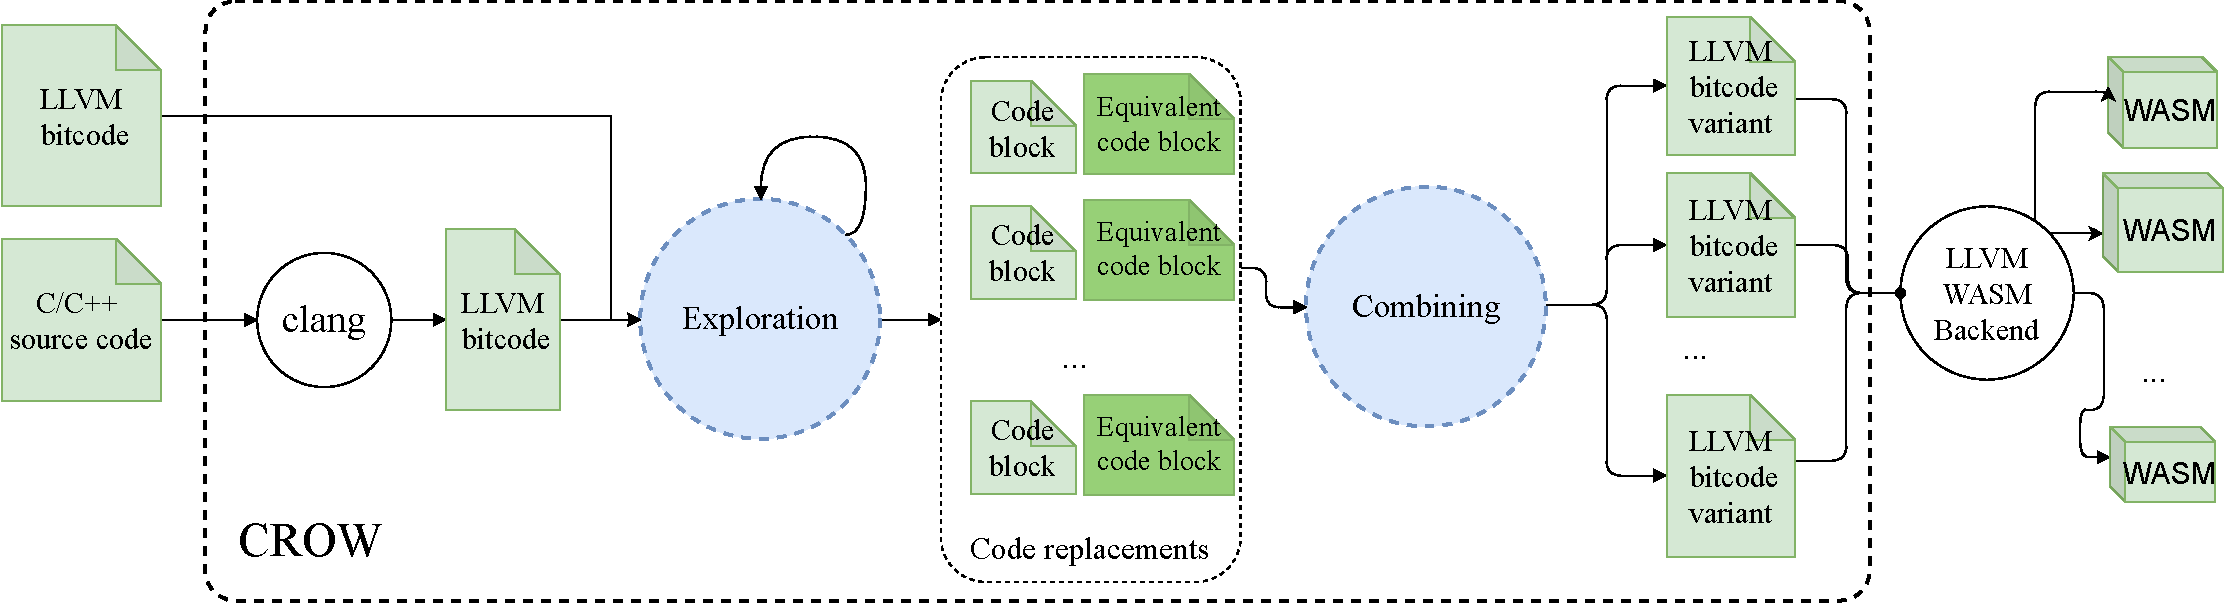
\includegraphics[width=\linewidth]{diagrams/generation/crow.drawio.pdf}
        \caption{CROW workflow to generate program variants. CROW takes C/C++ source codes or LLVM bitcodes to look for code blocks that can be replaced by semantically equivalent code and generates program variants by combining them.}
        \label{diagrams:crow}
    \end{figure*}
    
    Figure \ref{diagrams:crow} highlights the main two stages of the CROW's workflow, \textit{exploration} and \textit{combining}. The workflow starts by compiling the input program into the LLVM bitcode using clang from the source code. During the \emph{exploration} stage, CROW takes an LLVM bitcode and, for its code blocks, produces a collection of code replacements that are functionally equivalent to the original program. In the following, we enunciate the definitions we use along with this work for a code block, functional equivalence, and code replacement. 
    
    
    \begin{definition}{Block (based on Aho \etal \cite{10.5555/6448}):}\label{def:code-block}
        Let $P$ be a program. A block $B$ is a grouping of declarations and statements in $P$ inside a function $F$. 
    \end{definition}
    
    
    \begin{definition}{Functional equivalence modulo program state (based on Le \etal \cite{10.1145/2594291.2594334}):}
        \label{def:functional-equivalence}
        Let $B_1$ and $B_2$ be two code blocks according to \autoref{def:code-block}. We consider the program state before the execution of the block, $S_i$, as the input and the program state after the execution of the block, $S_o$, as the output. $B_1$ and $B_2$ are functionally equivalent if given the same input $S_i$ both codes produce the same output $S_o$.
    \end{definition}
    
    \begin{definition}{Code replacement:}
        \label{def:code-replacement}
        Let $P$ be a program and $T$ a pair of code blocks $(B_1, B_2)$. $T$ is a candidate code replacement if $B_1$ and $B_2$ are both functionally equivalent as defined in \autoref{def:functional-equivalence}.
        Applying $T$ to $P$ means replacing $B_1$ by $B_2$. The application of $T$ to $P$ produces a program variant $P'$ which consequently is functionally equivalent to $P$.     
    \end{definition}
    
    We implement the \emph{exploration} stage by retargeting a superoptimizer for  LLVM, using its subset of the LLVM intermediate representation. CROW operates at the code block level, taking them from the functions defined inside the input LLVM bitcode module. In addition, the retargeted superoptimizer is in charge of finding the potential places in the original code blocks where a replacement can be applied. Finally, we use the enumerative synthesis strategy of the retargeted superoptimizer to generate code replacements.
    The code replacements generated through synthesis are verified, according to \autoref{def:functional-equivalence}, by internally using a theorem prover. 
    
    Moreover, we prevent the superoptimizer from synthesizing instructions that have no correspondence in \wasm\ for the sake of reducing the searching space for equivalent program variants. Besides, we disable all optimizations in the \wasm\ LLVM backend that could reverse the superoptimizer transformations, such as constant folding and instructions normalization.
    
    %\todo{We disable cost restrictions and the LLVM backend optimizations...maybe for the assesment RQ ?}
    
    In the \emph{combining} stage, CROW combines the candidate code replacements to generate different LLVM bitcode variants, selecting and merging the code replacements. 
    Then for each combination, a variant bitcode is compiled into a \wasm\ binary if requested. Finally, CROW generates the variants from all possible combinations of code replacements as the power set of all code replacements.  
    
    \end{comment}


    % For presentation

\subsection*{CROW instantiation}
%\label{section:crow:example}
%In \autoref{section:crow} we describe the main components and contributions of CROW. In this section we instantiate the workflow presented in \autoref{workflow} from the input of an example C code to the generation of a pool of \wasm\ program variants.

Let us illustrate how CROW works with the simple example code in \autoref{CExample}. The \texttt{f} function calculates the value of $2 * x + x$ where \texttt{x} is the input for the function.  CROW compiles this source code and generates the intermediate LLVM bitcode in the left most part of \autoref{example:crow:original:llvm}. CROW potentially finds two integer returning instructions to look for variants, as the right-most part of \autoref{example:crow:original:llvm} shows.

% snippet of code showing the detection of code blocks
    
\begin{code}
    \lstset{language=C,
    basicstyle=\small\ttfamily,caption={C function that calculates the quantity $2x + x$},label=CExample}
    \begin{lstlisting}[style=CStyle]
int f(int x) { 
    return 2 * x + x; 
}    
    \end{lstlisting}
    
\end{code}

\lstdefinelanguage{LLVM}
    {morekeywords={i32,mul,align,nsw,add,load,store,define,br, ret, shl, ret},
    sensitive=false,
    morecomment=[l]{;},
    morecomment=[s]{;}{;},
    morestring=[b],
}
\lstdefinestyle{nccode}{
    numbers=left,
    tabsize=4,
    showspaces=false,
    breaklines=true, 
    showstringspaces=false,
    moredelim=**[is][{\btHL[fill=black!10]}]{`}{`},
    moredelim=**[is][{\btHL[fill=celadon!40]}]{!}{!}
}
\lstset{
    language=LLVM,
    style=nccode,
    %basicstyle=\small\ttfamily,
    columns=fullflexible,
    breaklines=true
}


\begin{code}
    \centering
    \captionof{lstlisting}{LLVM's intermediate representation program, its extracted instructions and replacement candidates. Gray highlighted lines represent original code, green for code replacements. }\label{example:crow:original:llvm}
    \lstset{numbers=none}
    \noindent\begin{minipage}[t]{.33\linewidth}
    \centering
    \begin{lstlisting}[xleftmargin=1em,escapechar=?]
    define i32 @f(i32) {

    ?\tikzmarkWS{2}{code 2}{11.5}{10}{3.5cm}?
    ?\tikzmarkWS{1}{code 1}{11.5}{3.5}{3.0cm}?
    %2 = mul nsw i32 %0,2
    %3 = add nsw i32 %0,%2 

    ret i32 %3
    }
    
    define i32 @main() {
    %1 = tail call i32 @f(i32 10)
    ret i32 %1
    }
    \end{lstlisting}
    \end{minipage}%\hfill%
    \begin{minipage}[t]{.32\linewidth}
        \begin{lstlisting}[xleftmargin=1em,escapechar=?]
?Replacement candidates for code\_1?

`%2 = mul nsw i32 %0,2`

!%2 = add nsw i32 %0,%0!

!%2 = shl nsw i32 %0, 1:i32!
    \end{lstlisting}
    \end{minipage}%\hfill%
    \begin{minipage}[t]{.32\linewidth}
        \lstdefinestyle{nccode}{
        tabsize=4, 
        showspaces=false,
        breaklines=true, 
        showstringspaces=false,
        moredelim=**[is][{\btHL[fill=black!10]}]{`}{`},
        moredelim=**[is][{\btHL[fill=celadon!40]}]{!}{!}
        }
        \lstset{
            language=LLVM,
            style=nccode,
            columns=fullflexible,
            breaklines=true,
            belowcaptionskip=1pt,
            abovecaptionskip=1pt,
        } 
        \begin{lstlisting}[name={B},escapechar=?]
?Replacement candidates for code\_2?

`%3 = add nsw i32 %0,%2`

!%3 = mul nsw %0, 3:i32!
        \end{lstlisting}
    \end{minipage}
    
\end{code}





\begin{code}
    \centering
    \captionof{lstlisting}{Candidate code replacements combination. Orange highlighted code illustrate replacement candidate overlapping.}\label{example:crow:original:combination}
    \lstset{numbers=none}
    \noindent\begin{minipage}[t]{.5\linewidth}
    \begin{lstlisting}[xleftmargin=1em,escapechar=?]
`%2 = mul nsw i32 %0,2`
`%3 = add nsw i32 %0,%2`

!%2 = add nsw i32 %0,%0!
`%3 = add nsw i32 %0,%2`

!%2 = shl nsw i32 %0, 1:i32!
`%3 = add nsw i32 %0,%2`

    \end{lstlisting}
    \end{minipage}%\hfill%
    \begin{minipage}[t]{.5\linewidth}
        \lstdefinestyle{nccode}{
        tabsize=4, 
        showspaces=false,
        breaklines=true, 
        showstringspaces=false,
        moredelim=**[is][{\btHL[fill=black!10]}]{`}{`},
        moredelim=**[is][{\btHL[fill=celadon!40]}]{!}{!},
        moredelim=**[is][{\btHL[fill=weborange!40]}]{'}{'}
        }
        \lstset{
            language=LLVM,
            style=nccode,
            columns=fullflexible,
            breaklines=true,
            belowcaptionskip=1pt,
            abovecaptionskip=1pt,
        } 
        \begin{lstlisting}[xleftmargin=1em,escapechar=?]
'%2 = mul nsw i32 %0,2'
!%3 = mul nsw %0, 3:i32!

'%2 = add nsw i32 %0,%0'
!%3 = mul nsw %0, 3:i32!

'%2 = shl nsw i32 %0, 1:i32'
!%3 = mul nsw %0, 3:i32!

    \end{lstlisting}
    \end{minipage}
\end{code}


\begin{tikzpicture}[remember picture,overlay]
%\path (2.north) edge[<-, bend left] (1.north);
%\path[draw, ->] (3.west) edge[<-, bend left] (2.west);
%\path (4.west) edge[<-, bend left] (3.west);
%\path (1.south) edge[<-, bend left] (4.south);

%\path (2.east) edge[<-, bend left, blue] (5.north);
%\path (3.east) edge[<-, bend right, olive] (2.east);
%\path (1.east) edge[<-, bend left, black] (replall1.west);
%\path (2.east) edge[<-, bend left, black] (replall2.west);
%\path (rep11.east) edge[<-, bend left, black] (6.east);
%\path (9.east) edge[<-, bend right, black] (4.east);
%\path (7.east) edge[<-, bend right, black] (8.east);
%\path (5.south) edge[<-, bend right, blue] (4.east);
%\path (9.north) edge[<-] (8.south);
%\path (5.south) edge[<-, bend left] (9.south);


%\path (10.north) edge[<-, bend left] (11.north);
%\path (11.south) edge[<-, bend left] (10.south);
%\path (7) edge[<-, bend right] (6.east);
%\path (8) edge[<-, bend right] (7.east);
\end{tikzpicture}


    

CROW, detects \texttt{code\_1} and \texttt{code\_2} as the enclosing boxes in the left most part of \autoref{example:crow:original:llvm} shows. CROW synthesizes $2 + 1$ candidate code replacements for each code respectively as the green highlighted lines show in the right most parts of \autoref{example:crow:original:llvm}.
The baseline strategy of CROW is to generate variants out of all possible combinations of the candidate code replacements, \ie uses the power set of all candidate code replacements.

In the example, the power set is the cartesian product of the found candidate code replacements for each code block, including the original ones, as \autoref{example:crow:original:combination} shows. The power set size results in $6$ potential function variants. Yet, the generation stage would eventually generate $4$ variants from the original program. CROW generated 4 statically different Wasm  files, as \autoref{example:crow:variants:wasm} illustrates. This gap between the potential and the actual number of variants is a consequence of the redundancy among the bitcode variants when composed into one. In other words, if the replaced code removes other code blocks, all possible combinations having it will be in the end the same program. In the example case, replacing \texttt{code\_2} by \texttt{mul nsw \%0, 3}, turns \texttt{code\_1} into dead code, thus, later replacements generate the same program variants. The rightmost part of \autoref{example:crow:original:combination} illustrates how for three different combinations, CROW produces the same variant. We call this phenomenon a \emph{code replacement overlapping}{Software!Replacement overlapping}.

\lstdefinestyle{nccode}{
        numbers=none,
        firstnumber=2,
        stepnumber=1,
        numbersep=10pt,
        tabsize=4, 
        showspaces=false,
        breaklines=true, 
        showstringspaces=false,
    moredelim=**[is][\btHL]{`}{`},
    moredelim=**[is][{\btHL[fill=black!10]}]{`}{`},
    moredelim=**[is][{\btHL[fill=celadon!40]}]{!}{!}
}

\lstset{
    language=WAT,
    style=nccode,
    basicstyle=\footnotesize\ttfamily,
    columns=fullflexible,
    breaklines=true
}


\begin{code}
    \centering
    \captionof{lstlisting}{\termidx{Wasm }program variants generated from program \autoref{CExample}.}\label{example:crow:variants:wasm}
    \lstset{numbers=none}
    \noindent\begin{minipage}[t]{.45\linewidth}
    \begin{lstlisting}[xleftmargin=1em,escapechar=?]
func $f (param i32) (result i32)
   local.get 0
    `i32.const 2`
    `i32.mul`
    `local.get 0`
    `i32.add`

        \end{lstlisting}
\begin{lstlisting}[xleftmargin=1em,escapechar=?]
func $f (param i32) (result i32)
    local.get 0
    !local.get 0!
    !i32.add!
    `local.get 0`
    `i32.add`

                \end{lstlisting}
    \end{minipage}\hfill
    \noindent\begin{minipage}[t]{.45\linewidth}
\begin{lstlisting}[xleftmargin=1em,escapechar=?]
func $f (param i32) (result i32)
    local.get 0
    !i32.const 1!
    !i32.shl!
    `local.get 0`
    `i32.add`

    \end{lstlisting}
\begin{lstlisting}[xleftmargin=1em,escapechar=?]
func $f (param i32) (result i32)
    local.get 0
    !i32.const 3!
    !i32.mul!

            \end{lstlisting}
        \end{minipage}
\end{code}




One might think that a reasonable heuristic could be implemented to avoid such overlapping cases. Instead, we have found it easier and faster to generate the variants with the combination of the replacement and check their uniqueness after the program variant is compiled. This prevents us from having an expensive checking for overlapping inside the CROW code. Still, this phenomenon calls for later optimizations in future works.


\subsection{Combining replacements}

When we retarget Souper, to create variants, we recombine all code replacements, including those for which a constant inferring was performed.
This allows us to create variants that are also better than the original program in terms of size and performance. Most of the Artificial Software Diversification  works generate variants that are as performant or iller than the original program. By using a superdiversifier, we could be able to generate variants that are better, in terms of performance, than the original program. This will give the option to developers to decide between performance and diversification without sacrificing the former. 

On the other hand, when Souper finds a replacement, it is applied to all equal instructions in the original LLVM binary. In our implementation, we apply the transformation only to the instruction for which it was found in the first place. For example, if we find a replacement that is suitable for $N$ difference places in the original program, we generate $N$ different programs by applying the transformation in only one place at a time. Notice that this strategy provides a combinatorial explosion of program variants as soon as the number of replacements increases.


\begin{comment}

    \subsection{Multivariant Binary Execution at the Edge}
    
    % \todo{Introduce as the use of MEWE}
    
    % What really is executed is the x86 code
    When a WebAssembly binary is deployed on an edge platform, it is translated to machine code on the fly.
    For our experiment, we deploy on the production edge nodes of Fastly. This edge computing platform uses Lucet, a native WebAssembly compiler and runtime, to compile and run the deployed Wasm  binary \footnote{\url{https://github.com/bytecodealliance/lucet}}.
    Lucet generates x86 machine code and ensures that the generated machine code executes inside a secure sandbox, controlling memory isolation.
    
    
    \begin{figure}
    \centering
      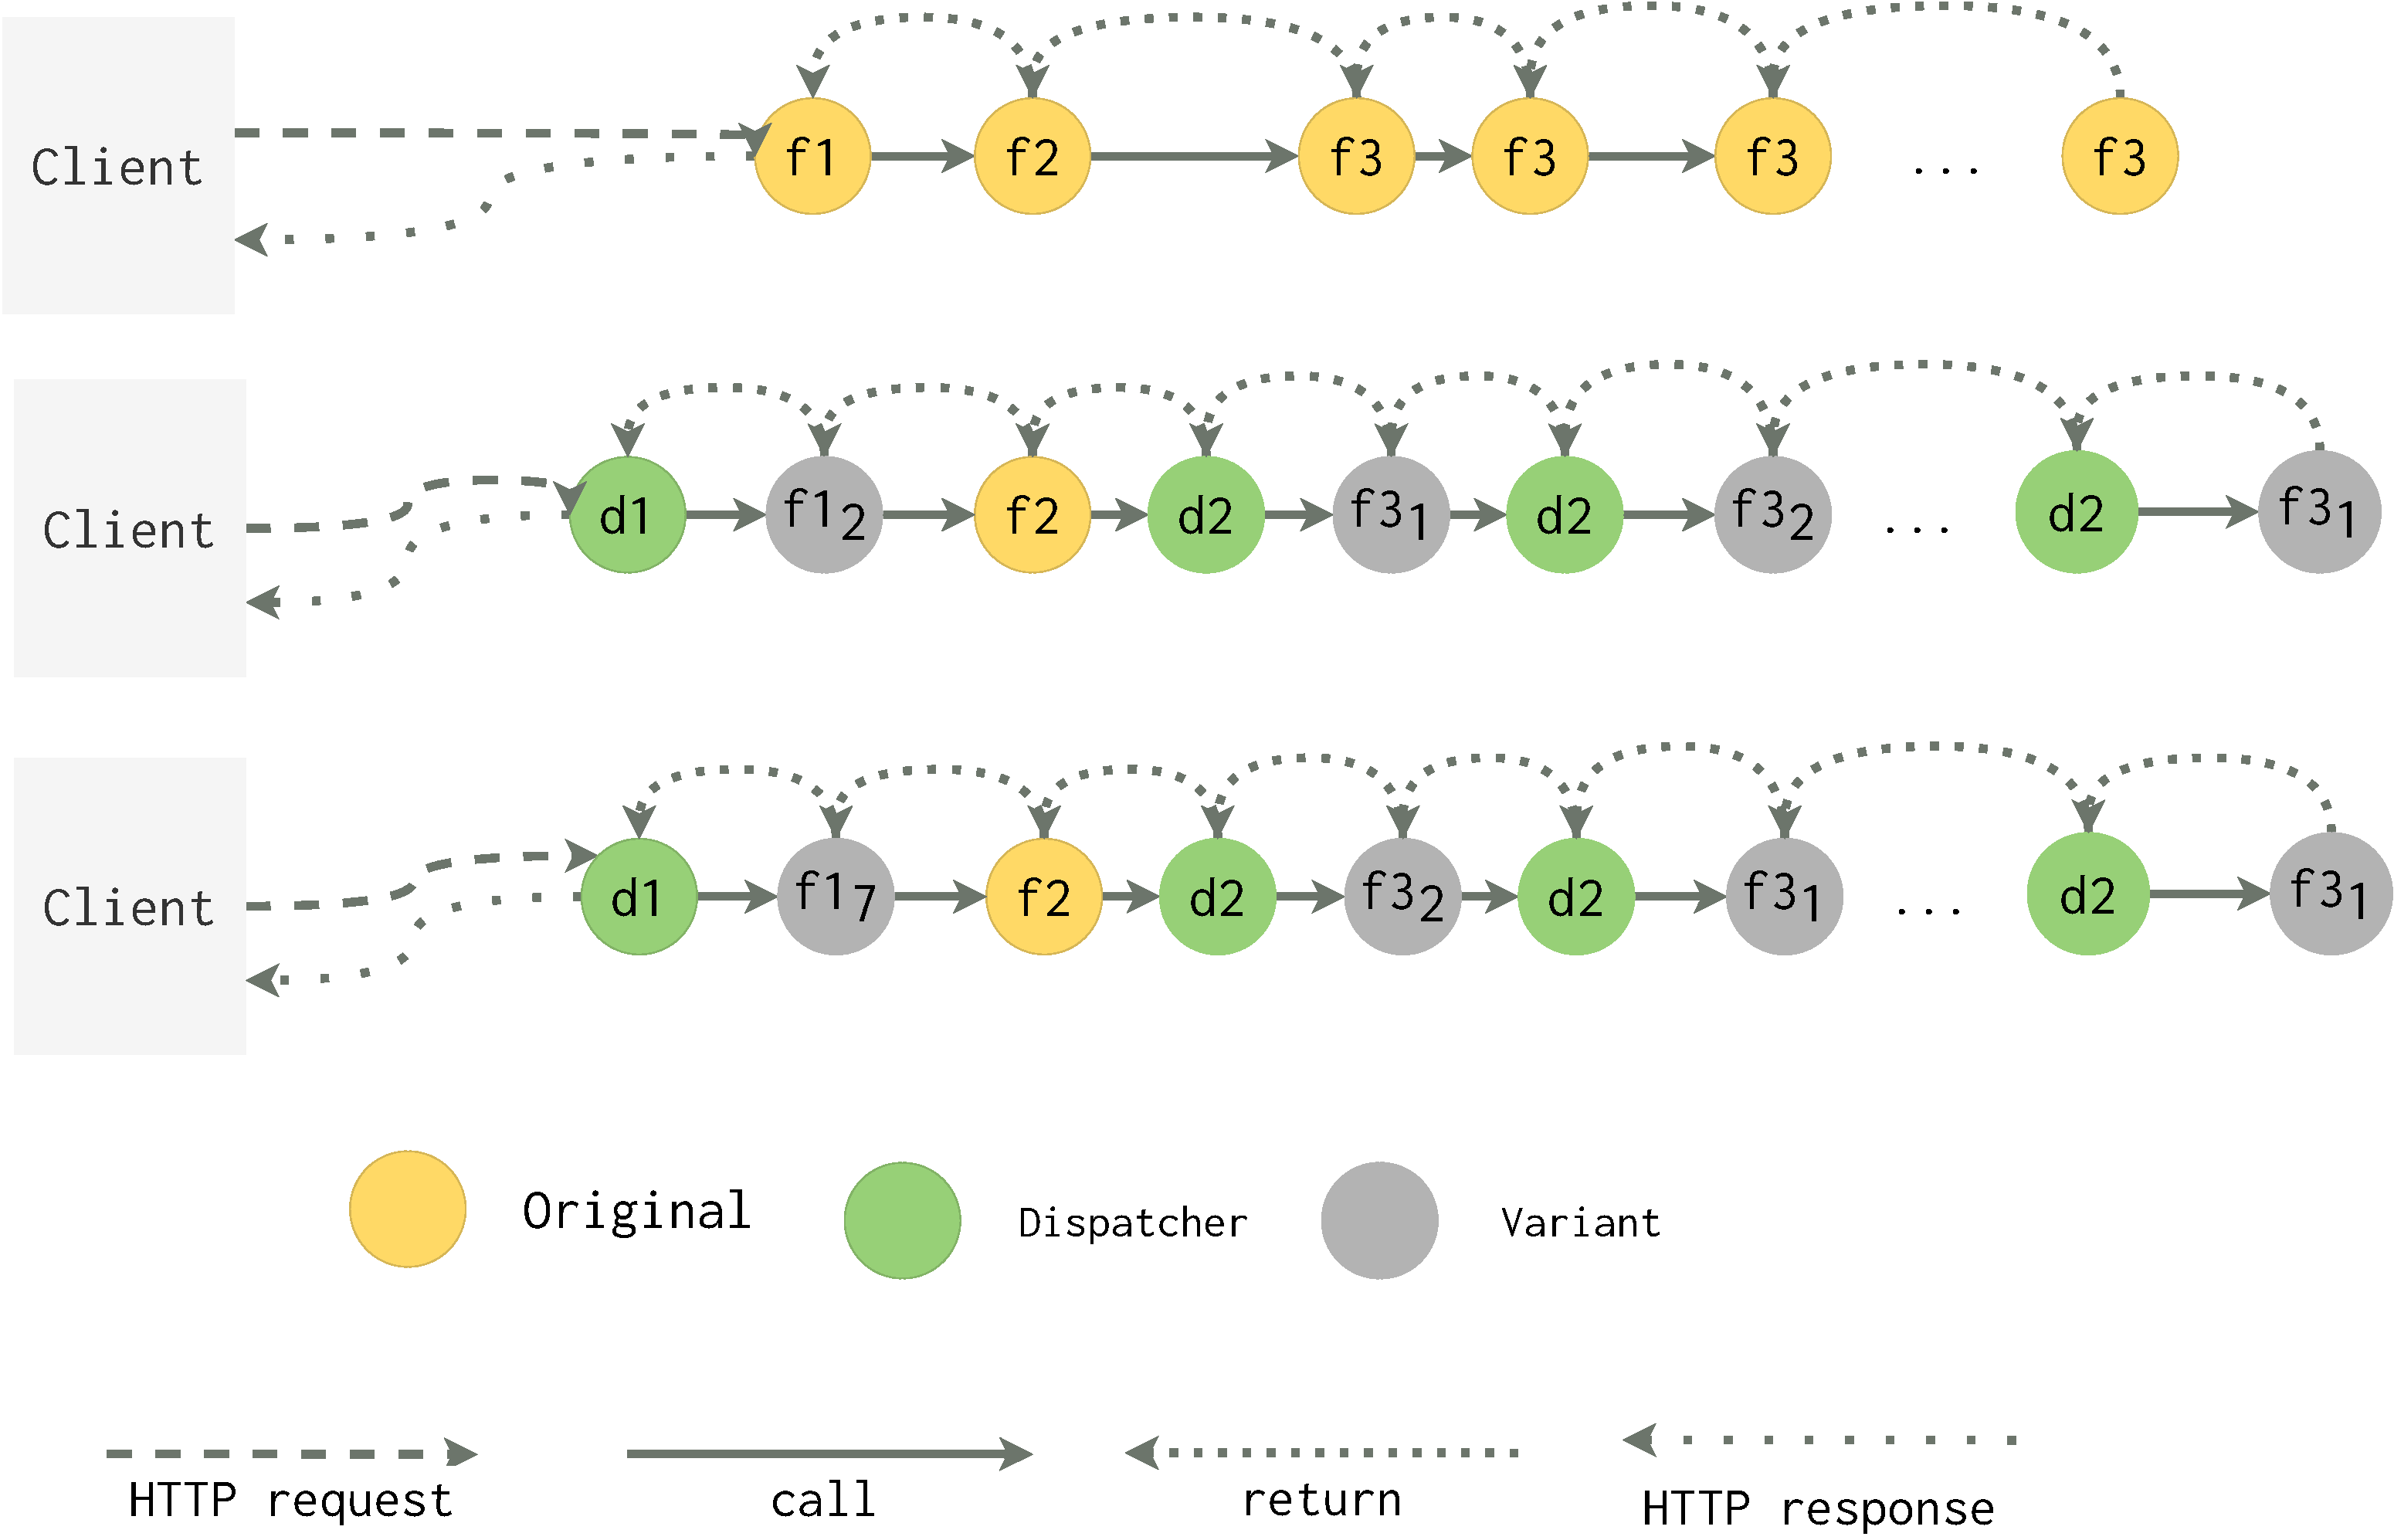
\includegraphics[width=1\linewidth]{diagrams/traces.pdf}
      \caption{Top: an execution trace for the  \texttt{bin2base64} endpoint. Middle and bottom: two different execution traces for the multivariant \texttt{bin2base64}, exhibited by two different requests with exactly the same input.}
      \label{http:workflow}
    \end{figure}
    
    % How it works
    \autoref{http:workflow} illustrates  the runtime behavior of the original and the multivariant binary,  when deployed on an Edge node.
    The top most diagram illustrates the execution trace for the  original of the endpoint \texttt{bin2base64}.
    When the HTTP request with the input \texttt{"Hello World!"} is received, it invokes functions $f1$, $f2$ followed by 27 recursive calls of function $f3$. Then, the endpoint sends the result \texttt{"0x000xccv0x10x00b3Jsx130x000x00 0x00xpopAHRvdGE="} of its base64 encoding in an HTTP response.
    
    The two diagrams at the bottom of \autoref{http:workflow} illustrate two executions traces observed through two different requests to the endpoint \texttt{bin2base64}.
    In the first case, the request first triggers the invocation of dispatcher $d1$, which randomly decides to invoke the variant $f1_2$; then $f2$, which has not been diversified by \tool, is invoked; then the recursive invocations to $f3$ are replaced by iterations over the execution of dispatcher $d2$ followed by a random choice of variants of $f3$. Eventually the result is computed and sent back as an HTTP response. 
    The second execution trace of the multivariant binary shows the same sequence of dispatcher and function calls as the previous trace, and also shows that for a different requests, the variants of $f1$ and $f3$ are different. 
    
    
    The key insights from these figures are as follows. First, from a client's point of view, a request to the original or to a multivariant endpoint, is completely transparent. Clients send the same data, receive the same result, through the same protocol, in both cases.
    Second, this figure shows that, at runtime, the execution paths for the same endpoint are different from one execution to another, and that this randomization process results from multiple random choices among function variants, made through the execution of the endpoint.
    %From an attacker's perspective, this random selection of variants constantly moves the attack surface and is meant to render a potential vulnerability harder to reach or exploit \cite{davi2015isomeron, 10.5555/3091125.3091155, BEKIROGLU2021106601}.
    
    
    \end{comment}
    